\documentclass[nobiblatex]{LTHthesis}
% !TeX spellcheck = en_GB
\usepackage[T1]{fontenc}
\usepackage[utf8]{inputenc}  %% Comment if you are not using utf8
\usepackage{mathptmx, helvet}
\usepackage{xfrac}
%\usepackage[swedish]{babel}  %% aktivera om rapporten är på svenska
\usepackage[left=2.5cm,right=2.5cm,top=3cm,bottom=5cm]{geometry}
\usepackage{graphicx}
\usepackage{listings}
\usepackage{url}

\usepackage{titlesec}
\usepackage{todonotes}

\newcommand{\martina}[1]{\todo[inline,color=red!30,caption={}]{\textbf{Martina:} #1}}


\begin{document}
\begin{titlepages}
\author{Fredrik Johnsson and Olle Svensson}
\title{Resource management and prioritization in an embedded Linux system}
\year{2014}
\month{June}
\TFRT{9999}  %%  You will get the number from the department.
\printer{Media-Tryck}  %% Probably. You may get other information from the department.

\end{titlepages}
\setcounter{page}{1}
\pagenumbering{roman}

\chapter*{Abstract}
This master thesis report will depict the work carried out at Axis Communications in cooperation with the Department of Control at Lunds University. The problem of limited resources on an Axis camera is handled by a two
part solution where a resource manager (RM) distributes the available re-
sources and where services adapt their service level (SL) in order to let the
services finish their jobs on time. This is done in a game theoretic approach
where the services are players, varying their SL in order to get a good match
between given resources and their SL. This SL-adaptation scheme is then
implemented on the streaming service on the camera and on some test ser-
vices performing simple math operations. The resource manager is incor-
porated into systemd which uses CGroups [1] to implement the distribution
of resources.


\chapter*{Acknowledgements}
We want to thank our supervisors, Umut Tezduyar-Lindskog, Axis and Martina Maggio, LTH Department of Control. We would also like to thank engineering manager Pontus Bergendahl, Axis.

\newpage
\tableofcontents
\newpage

\setcounter{page}{1}
\pagenumbering{arabic}

\chapter{Introduction} %This is a description of my work.
\section{Axis}
Axis is a company founded and based in Lund that manufactures network relayed surveillance cameras and video encoders.
\section{Problem formulation}
It is becoming more common to have multiple resource intensive services running on Axis cameras. At the same time, the demands are increasing on reliable and consistent video frame rate and quality. This creates a problem where different services are competing for resources like CPU and RAM. This can result in poor performance of the camera under scenarios when it is under heavier load than usual, one example being when answering calls from the network. The solution that we will evaluate is based on some of the work carried out at the University of Lund \cite{gtrm}, called the Game Theoretic Resource Manager (GTRM) and a library that lets services implement the SL adaptation and communication with the RM. The goal is to see if it is possible to use this resource manager on an Axis camera running Linux with the streaming application competing with some test applications for resources. In this test the cameras image quality will be its SL and the inverse of its frame rate the measurement for the time a job takes to finish, where a jobs deadline will be set to \(1/desired framerate\).


\section{Related Work}

\martina{Rephrase this}

Resource management is a problem that can be solved in many different ways. Many resource managers has been developed in the past and also some with game theoretic behavior.  

The problem of allocating resources to, assumed, fully parallelizable tasks was solved by Wei et al.~\cite{Wei10} using a game-theoretic method.

Subrata et al.~\cite{Sub08} solved the problem of balancing the load in grid computing by applying game theory. Here the players are machines that wants to maximize their profit by finishing jobs that arrive according to a Poisson process.

Grosu and
Chronopoulos~\cite{Gro05} made similar work with load balancing. Here the load was distributed amongst different competing players which would hopefully reach a common state which would benefit all the players the most.

Many resource managers are feedback oriented and resource allocation using feedback loops was developed by Lu et al.~\cite{LuS99a},
Steere et al.~\cite{Ste99}, Eker et al.~\cite{Eke00}. However they do not implement the concept of altering quality.

The QoS-based Resource Allocation Model (Q-RAM) was proposed by Rajkumar et al.~\cite{Raj97a} for managing of multidimensional resources. Here it is desired to minimize the QoS constraints while maximizing the \emph{total utility}. 
 
A solution that both manages the resources and the service level of an application is proposed in the ACTORS project ~\cite{Bin11}, but just as the solutions proposed by \cite{Raj97a,Soj11,Arz11} this is done in a centralized way. 

Separating the service-level adjustment and the resource management has been proposed to solve network bandwith allocation, ~\cite{Sil11}.

% Instead, we believe that the assignment of the service level can be
% better performed by the application itself, rather than at a
% centralized resource management level.

\martina{End of rephrase}

\section{Outline of the report}
Chapter 2, Background, will give a detailed description on the software and hardware used during this project.
Chapter 3, Implementation, is about how development went fourth, what decisions were made and how the resulting product is composed.
Chapter 4, Use cases, this chapter describes the use cases that where presented during the project. These bring knowledge about what the product is supposed to do and not to do, and also what would be relevant to test in the finished prototype.
Chapter 5, Testing, how and what was tested in the product.
Chapter 6, Results, what results that could be extracted from this thesis.
Chapter 7, Conclusions and Further Work, what could be concluded from the result and what could be improved given more time.
\chapter{Background}

\section{Game Theoretic Resource Manager}
The resource management is based on the performance of the applications that are running. By calculating the difference between the applications deadline and its execution time one gets the performance, also called matching function, of the application. Ideally the matching function should be zero. When zero, the  application has just enough resources to meet its deadline running with some SL. When positive, too much resources are assigned to the application, indicating that the job is done before deadline, and when negative, too little resources are assigned indicating that the application has missed its deadline.

The resource managing consists of two parts:
\subsection{Service Level adaptation}
The Service Level (SL) defines the quality of service of the application. In the case of the streaming application this is the quality of the image, but it can mean different things to different applications. The main property of the SL is that an increase in SL gives an increase in the required resources for the application. The idea is to change the SL to optimize the utilization of the amount of resources available. A high/low performance will be responded to by an increase/decrease in SL.
This will make sure that the application is always presenting valid result in time but with quality as a trade-off. This adaptation is done by the application itself.

\subsection{Resource Manager}
The resource manager(RM) will also measure the performance of the applications. It will try to distribute the resource in the best possible way to the applications. The resources are modelled as “virtual platforms”, and is basically a percentage of the total available resources. For example the amount of time an application is allowed to use the CPU in proportion to the other applications. Here “resources” could refer to something other than CPU, such as memory or network-resources, depending on different aspects of the system. The main property of the performance is that if an application is given more/less resources it should be able to execute at a higher/lower SL or have a shorter/longer execution time.

The theory of decoupling the resource manager from the service level adaptation was developed at the Department of Automation at Lunds University. The resulting resource manager is referred to as Game Theoretic Resource Manager, GTRM. 

The idea behind this way of using a resource manager (RM) and service level (SL) adaptation, separating it from the norm, is to let each application adapt its own SL continuously independent from the RM loop. One of the main benefits of this decoupling is that the task of adjusting SL is given to the applications that have the most knowledge of how to tune their parameters in order to adjust their needed resources, and at what cost in quality.

\section{systemd and cgroups}
Systemd [sysd] is a system management daemon for Linux and it is the first process that starts during boot and thus it is given the PID number 1. Systemd implements a lot of features for increased performance and system management. It also has different features for management of resources, using cgroups \cite{cgroups}, which makes it interesting for our project. 

Cgroups, abbreviated from control groups, can be used to set the amount of resources, such as CPU or memory, of a process or a group of processes via a virtual file system. This file system forms a tree where the resources of a parent folder are shared by its children. The division of the resources among the children are determined by the amount of "shares" the children has been given. 

Each application can be run as a "service" by specifying a service file which defines many different parameters and options. In this file we can specify which application or applications should be associated with which service and for example how much CPU shall be given to this service. The service file can then be placed in a certain folder in the cgroup file hierarchy, see fig~\ref{ctree}. Different folders are used to represent different cgroup controllers or a different combination of controllers. Depending on which controllers are enabled different features are available, such as limiting CPU- and memory.   
 Services can be grouped into different slices and share properties depending on which slice they belong to.  
One can for example set how much CPU-time that shall be given to the applications in the slice and decide how the applications will divide it amongst themselves.



\subsection{CPUShares and the cgroups tree}
In this implementation of the \emph{GTRM}, the resources are divided using the CPUShares property of the \emph{slices} or \emph{services}, both special cases of the base type \emph{units}. Every slice is represented by a folder in the cgroup tree and has a CPUShares property that decides how much of the available resources of the parent slice it will get. A slice contains services and services contains applications. 
All the resources of a parent slice will be divided to the units under it according to how much shares they each have. A unit that has a third of the total shares of all units  on the same level under its parent slice will receive a third of the parents available resources and so on. An example of this is shown in fig \ref{fig:ctree} and fig \ref{fig:ctable}. Note that the top level folder in this example,the controller named CPU, is alone on its level meaning that the CPUShares for this slice don't matter since there is no competition.


\begin{figure}
\centering
\begin{picture}(200,200)
\put(95,130){\framebox(40,30){CPU}}
\put(115,130){\line(-2,-1){40}}
\put(115,130){\line(2,-1){40}}
\put(55,80){\framebox(40,30){Slice 1}}
\put(135,80){\framebox(40,30){Slice 2}}
\put(75,80){\line(-2,-1){40}}
\put(75,80){\line(2,-1){40}}
\put(15,30){\framebox(40,30){Service 1}}
\put(95,30){\framebox(40,30){Service 2}}

\end{picture}
\caption{The slices and services in the cgroup tree.}
\label{fig:ctree}
\end{figure}



\begin{figure}

\centering
\begin{tabular}{|c|c|c|} \hline
\emph{Name} & \emph{CPUShares} &  \emph{\% of CPU} \\ \hline
CPU & 1 & 100 \\ \hline
Slice 1 & 400 & 80 \\ \hline
Slice 2 & 100 & 20 \\ \hline
Service 1 & 200 & $2/3 * 80 = 53$ \\ \hline
Service 2 & 100 & $1/3 * 80 = 27$\\ \hline
\end{tabular}
\label{fig:ctable}
\caption{Table over assigned CPU for the different units.}

\end{figure}

\section{Video Streaming}
The video streaming is based upon the GStreamer multimedia framework. This is a modular system where a chain is built by linking elements together in a pipeline to form a process chain. Data flows downstream from a source element, through filter elements to finally end up in a sink element, see fig\ref{fig:pipeline}. The data is contained in buffers, which can contain one or more frames, flowing downstream. On the Axis camera the source element will receive the images already compressed by external hardware through another application which reads a file descriptor in order to get the frames from the encoding device. The data is then sent through a number of filters and is finally sent onto the network by the sink element. This chain is dynamically created depending on different settings like codecs used \emph{(jpeg,h264,...)}, or network connection \emph{(http or udp)}.
	

\begin{figure}
\begin{framed}
\label{fig:pipeline}
\begin{picture}(100,60)
\put(0,60){Pipeline}

\put(0,4){\framebox(50,50){Source}}
\put(50,29){\vector(1,0){50}}
\put(100,4){\framebox(50,50){filter}}
\put(150,29){\vector(1,0){50}}
\put(200,4){\framebox(50,50){Sink}}
\end{picture}
\end{framed}

\caption{The GStreamer pipeline.}
\end{figure}


\section{Sockets and epoll}
\subsection{Sockets}
The communication between services and systemd is done with sockets and since the RM will run in the systemd main loop this is the communication that will be used to send data between the applications and the RM.
Sockets are the endpoints for IPC \emph{(inter-process communication)} flows over a network,
where the processes may reside on the same computer or just on the same network. These sockets are provided by the socket() system routine in linux which can be interacted with through calling functions in api header files. An analogy for sockets are physical ports on a computer and a printer where the wire in between is the channel.
A call to the socket() api function creates a socket and returns an integer, a \emph{file descriptor},  which is unique for the socket and is used for referring to the sockets in future calls. A file descriptor \emph{(fd)} in Linux is associated with an open file, where the file can be anything that can be written to or read from. Having the fd gives access to read and write to/from the socket.
A socket can be of the type \emph{stream} or \emph{datagram}, the latter is used by the gtrm socket.
\subsection{epoll}
Epoll is a linux system call that allows the user to listen to multiple sockets simultaneously. This is done by calling the api function epoll\_wait(...) which returns a queue of event-objects containing information about what fd:s that has received datagrams together with other misc. information. By looking at this queue the user knows what fd:s to read with the read(...) function.  


\section{Equipment} %Description of camera and such
During the project we used two different cameras, the M1033 and the P3367, both manufactured by Axis. We first started using the M1033 because it came with systemd but we later switched to the P3367 because it ran a later version of systemd.

\subsection{Axis M1033}
\begin{figure}
    \centering
    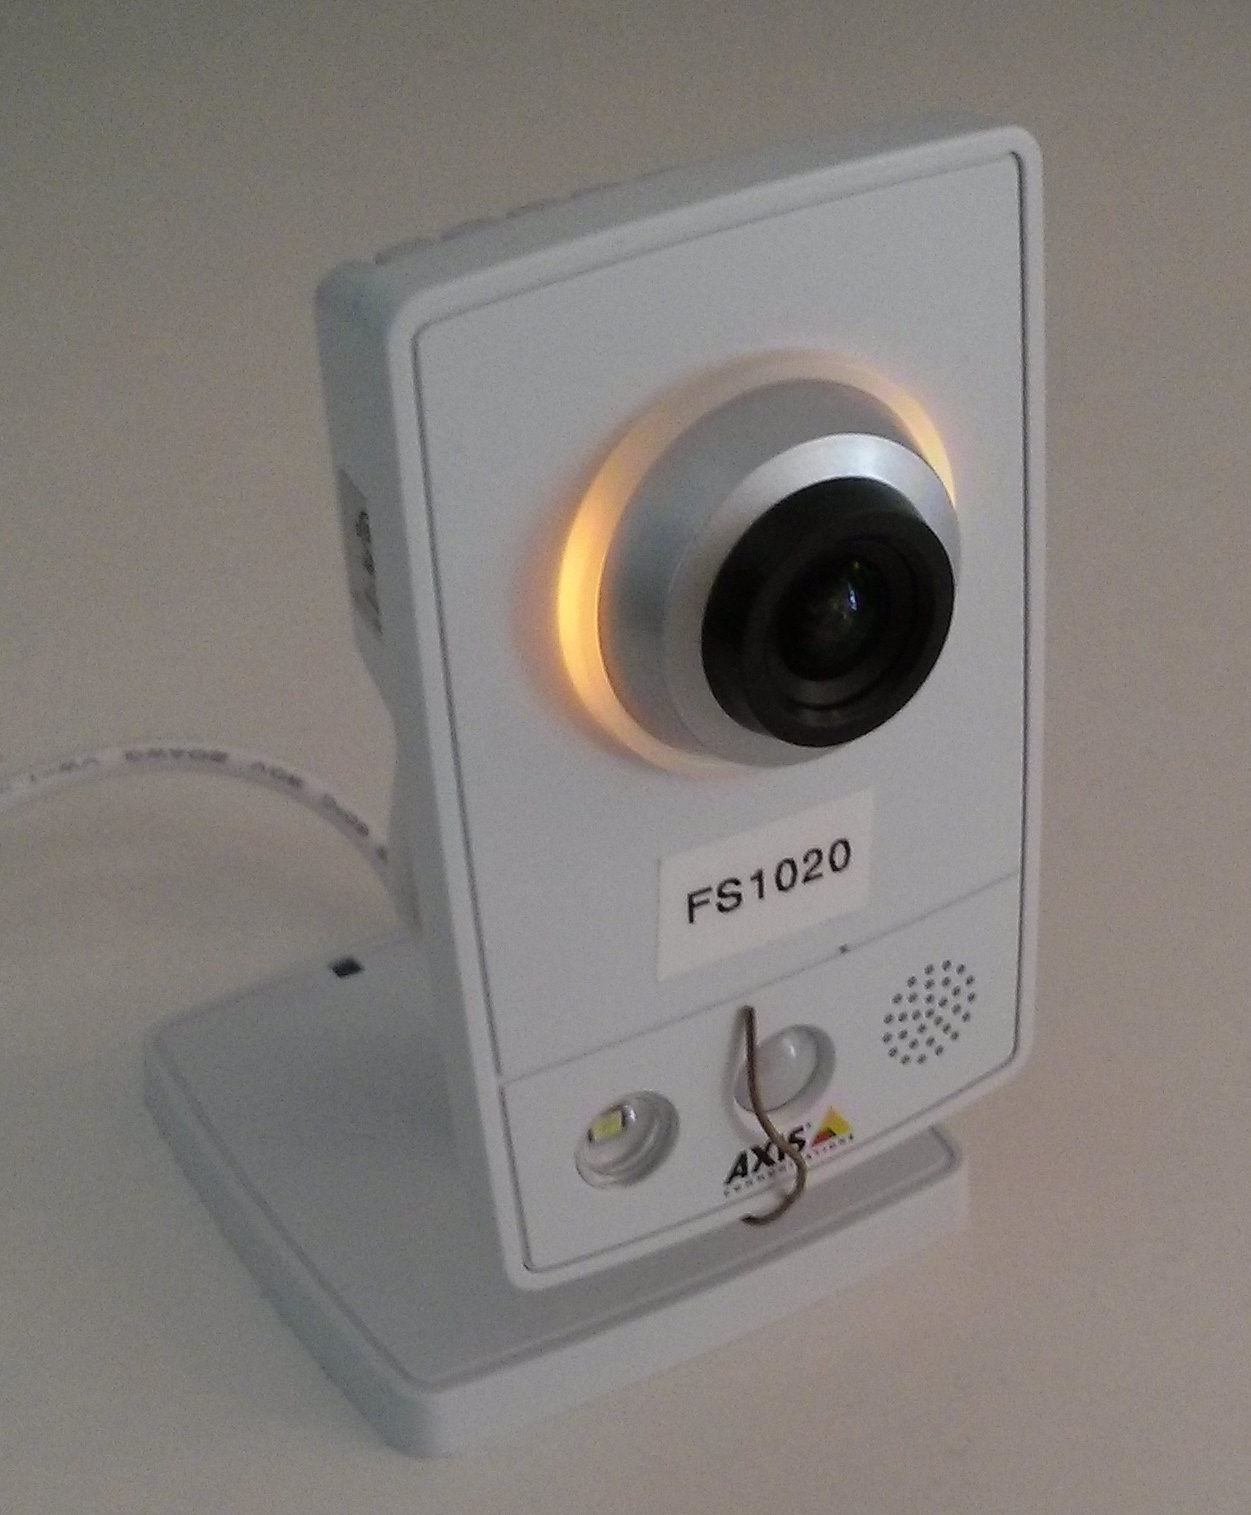
\includegraphics[width=\textwidth]{m1033}
    \caption{Axis M1033}
    \label{fig:M1033}
\end{figure}
This is a small camera, connected to the network either wired or wireless. It supports multiple H.264 streams and Motion JPEG running at a maximum resolution of 800x600 at 30 FPS. It has two way audio streaming, which means it can both record and play audio clips.

\subsection{Axis P3367}
\begin{figure}
    \centering
    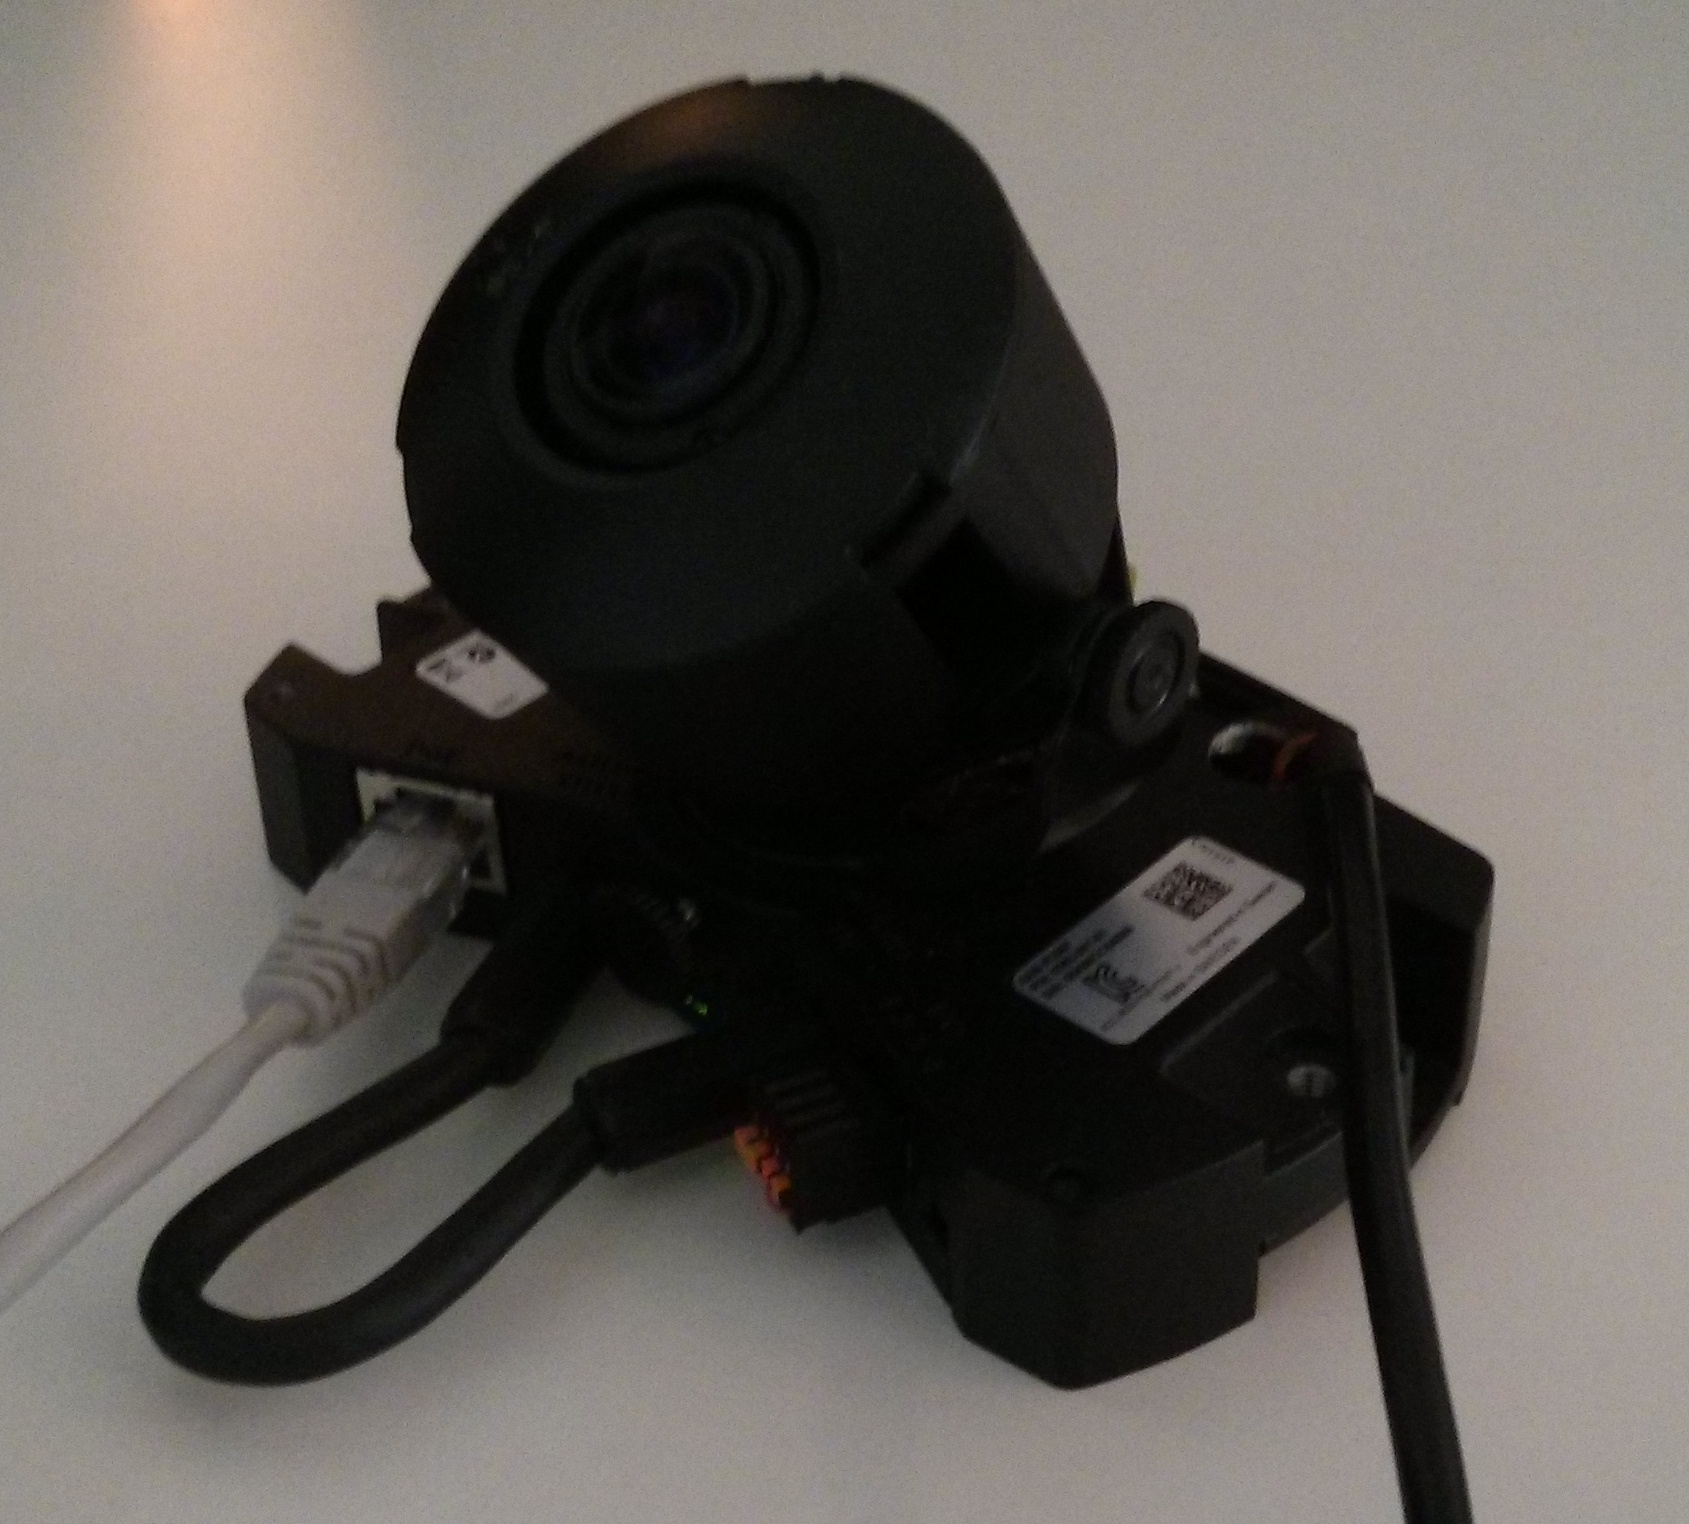
\includegraphics[width=\textwidth]{p3367}
    \caption{Axis P3367, without its casing}
    \label{fig:P3367}
\end{figure}
The Axis P3367 is a fixed dome network camera capable of multiple H.264 streams as well as Motion JPEG streams. It supports various frame rates and resolutions up to 5 MP at 12 FPS, it also supports HDTV 1080p at 30 FPS and has two way audio streaming capabilities. The power is supplied using Power over Ethernet, meaning it does not need a separate power supply, but is instead powered directly from the network cable. It features an ARTPEC-4 system-on-chip, developed by Axis, which contains a single-core CPU running at 400 MHz and a co-processor dedicated to video analytics.
\chapter{Implementation}
All code were written in C and cross-compiled using Axis' compiler for the corresponding platform e.g. camera. For the resource allocation different service files and slices were specified, and the resulting plots were generated with Octave.
\section{Constraints} %What we decided to do and not to do
Creating service levels for all the applications running on the system would not be a realistic approach. This is because there are many different applications, some of which may not even be developed at Axis, and developers cannot be expected to modify all of them to implement the performance measurements and service level features needed. Instead the service level part is only implemented in the video streaming application and on some test applications that does some random computations to stress the system. This thesis only focuses on the implementation of the already mentioned work at LTH and will not look into proofs of convergence for the algorithm, neither will it look into other types of SL functions than the simple linear case where the CPU requirement are a linear function of the SL. It can be argued that the CPU requirement/SL relationship can be linearized around a point and hence still be linear in a small intervall.

\section{Resource Management} 
The resource management is implemented as a part of systemd, with all of the resource management source code integrated into systemds. If an application has a poor matching function it sends this information to systemd via UNIX-sockets. Sockets represent an endpoint of communication and from these we can obtain a socket descriptor. These are used in the same way as file descriptors by the applications [socket]. Our interprocess communication (IPC) consists of a socket in systemd and one for each application that we are monitoring. From these sockets we can read or write messages between the applications and systemd. This was implemented by more or less copying the “Notify” feature of systemd which is used by certain applications that want to for example notify systemd that they have started or other status changes [sysd-notify].

The whole chain from the application to systemd is pretty long but most of it is managed in “sd-event” which serves as a wrapper around many different IPC events and messages. Our data transferred via sockets is picked up with the help of epoll, which is handled in sd-event. From this we can be notified and read data from the socket descriptor as soon it is available, in an interrupt based fashion. Finally we execute our dispatch function, which we register when the socket communication is established, and contain all the code that we want to execute when we receive a message to our socket. The function first extracts the data from the message, which is the PID of the sending application, its performance, whether it is satisfied or not and the weight attribute. We then update a hashmap which contains all our applications that are managed by GTRM. This data is then used when we calculate the virtual platforms and set the CPUShares in systemds “main-loop”.

\section{Service Level}
There are two ways of implementing SL, one simpler and one more advanced. The first one simply multiplies the current SL with the matching funtion and multiplies the result with a constant scale factor. This will decrease the service level if the performance i negative and increase it if it is positive. The scaling factor (called epsilon) also makes sure that we don't get too much overshoot. 
\[sl_i(t+1)= sl_i(t) + \epsilon*(f_i(t)*sl_i(t)) \]
The way also includes how much the virtual platform of the application has changed. This is calculated as the performance multiplier, PM.
\[PM_i = (1+f_i)*(vp_i(i+1)/vp(i))\]
After calculating the performance multiplier the new service level can be calculated like this
\[sl_i(t+1)=sl_i(t) + (\epsilon*sl_i(t)*PM_i)\]
\section{Resource Allocation}
\begin{figure}
    \centering
    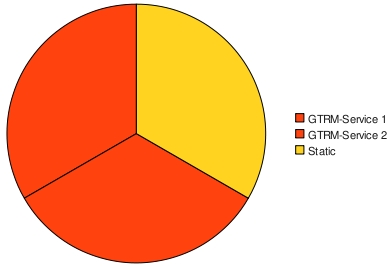
\includegraphics{piechart.jpeg}
    \caption{Pie chart describing how we split up our resources}
    \label{fig:Piechart}
\end{figure}
Using slices we can set a minimum amount of available resources for the applications in the slice. If the applications under a slice/service don’t use all of the resources given to them, the unused resources are free to be used by other slices. Under each slice there can be sub-slices or services dividing the resources further, building a hierarchy in the cgroups folder. The slices in the pie chart above, represent two different sets of applications. The static green slice consists of applications that won’t be managed by GTRM and simply will share the resources under this slice according to a predefined setting. Good choices of applications to put here would be ones that doesn’t vary much in their resource requirements or ones that have very strict hard deadlines. The second slice, the red GTRM slice, consists of applications that will be managed by the GTRM and that might implement SL adaptation. Good choices of applications to put here would be ones that do vary much in their resource requirements and/or can vary it’s quality in some acceptable way to adapt to it’s available resources.

All applications that are managed by the GTRM are run as services under the GTRM-slice. A service can, just as a slice, reserve a minimum percentage of allocated resources from it’s parent slice.

In the Pie chart above the static slice would be guaranteed a minimum of \sfrac{1}{3} of the total resources while Service1 and Service2 would be given half of the \sfrac{2}{3} reserved by its parent slice, guaranteeing  them a minimum of \sfrac{1}{3} of the total available resources each.

The resources of the applications running in the GTRM-slice will be managed by our GTRM. Some of the applications will have SL capabilities implemented and some will not. The reason for this is mainly because of the scope of our project. We are mainly concerned about using the SL to maintain a steady framerate but ideally all applications running in the GTRM-slice should, if it makes sense to the application, have a SL implemented to put the theory into practice. An extension of the project would be to have the entire system managed by the GTRM and have all applications manage their SL. The weight is the parameter that sets how big part of the adaptation that is made by changing the service level contra changing the amount of resources. By using the weight parameter we can make up for the fact that we can’t change SL of some applications and the GTRM will only manage their resources instead. 

\section{Source Code}
\begin{figure}
    \centering
    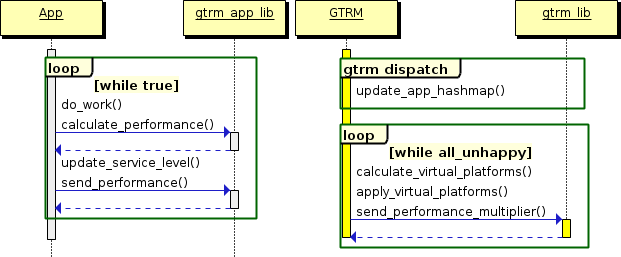
\includegraphics[width=\textwidth]{diag.png}
    \caption{Sequence diagram}
    \label{fig:sdiag}
\end{figure}
The sequence diagram in figure \ref{fig:sdiag} describes the flow of execution throughout the system via pseudo-code. Some functions call that are not relevant have been left out but will be described further below. 

The first important part in the application is the calculation of its performance, the matching function, here called \emph{calculate\_performance()}. The matching function has to be properly calculated or else the application will not be managed correctly. According to this matching function the service level will then be adapted, \emph{update\_service\_level()} and finally the resource manager will be notified by the \emph{send\_performance()} call.

The resource manager part basically consists of two parts that sort of runs in parallel. Upon receiving the performance of an application, the handler or dispatch function corresponding to such an event is executed. In the diagram it is labled as \emph{gtrm\_dispatch}, and its main responsibilities is to read and parse the received message and then update the hash-map which contains the relevant data about the applications being managed. Meanwhile the resource management runs as a part of the main-loop, and it uses the information in the hash-map previously mentioned to calculate the virtual platforms, \emph{calculate\_virtual\_platforms}. These virtual platforms are then used to set the amount of CPUShares which will be given to each application in the call to \emph{apply\_virtual\_platforms}. To get a better service level adaptation, the performance number which depends on how much the virtual platform has been changed is sent to the application \emph{send\_performance\_number}.

The system is implemented by the functions described in the following source and header files. Note that some of these files originate from the source of systemd and have only been edited and not created by the authors.

\subsection{manager.c/h}
\subsubsection{static int manager\_dispatch\_gtrm\_fd(sd\_event\_source *source, int fd, unit32\_t revents, void *userdata)}
\begin{itemize}
\item Called when we receive the performance of an application.
\item source: source of the event.
\item fd: file descriptor to the event source.
\item revents: ???
\item userdata: In this case it contains a reference to the manager.
\item Return value: Not used, always zero.
\end{itemize}

\subsubsection{static int manager\_setup\_gtrm(Manager *m)}
\begin{itemize}
\item Used to setup the socket, event source and file descriptor for the resource manager.
\item m: Reference to the manager.
\item Return value: Zero if function ran correctly, otherwise it is set to the corresponding error number.
\end{itemize}

\subsubsection{int gtrm\_compute\_virtual\_platforms(Hashmap *apps, gtrm\_t *gtrm\_t)}
\begin{itemize}
\item Calculates the amount of resources (virtual platform) for an application.
\item apps: The hash-map containing information about the applications being managed.
\item gtrm\_t: Struct with parameters used when calculating the virtual platforms.
\item Return value: Not used, always zero.
\end{itemize}

\subsubsection{void gtrm\_apply\_virtual\_platforms(Manager* m)}
\begin{itemize}
\item Computes and applies the amount of CPUShares that each application shall be given.
\item m: Reference to manager, used to get the applications
\item Return value: None.
\end{itemize}

\chapter{Use cases}
For implementation and testing reasons we came up with the following use-cases. In all the use cases we assume that the static slice is under heavy load so that no extra resources are given to the GTRM-slice. 
\section{Normal mode}
\begin{enumerate}
\item The system runs under good conditions, meaning we have enough resources for all applications and the GTRM-slice can run at maximum SL without any problems.
\item The GTRM and SL adaptation will not drag down performance compared to the old system.
\end{enumerate}
\section{Balancing a high load caused by video streaming}
The applications mentioned here are all on the GTRM-slice.

\begin{enumerate}
\item The camera will film something that causes a high load, for example, a PTZ-camera is moving around or an intense scenery is being filmed.
\item The applications with the worst performance  will adapt and lower their SL (e.g. quality) assuming they have weights setup to do so.
\item The GTRM will increase the resources given to the applications with the worst performance. These resources are taken from other, better performing,  processes on the slice that in turn will lower their SL to accommodate for the change in CPU.
\item When the scenery is “calmer” we will have an overall increase on the SL and the virtual platform will be redistributed.
\item The frame rate will be about the same during the entire procedure.
\end{enumerate}
\section{Balancing a high load caused by other applications}
In this case the static slice starts out not being under full load.
\begin{enumerate}
\item The static slice is giving extra resources to the GTRM-slice, making the applications on the GTRM-slice have a higher SL than they normally would.
\item The resource demand of the applications on the static slice starts to grow. 
\item The SL of the applications on the GTRM-slice will adapt and lower their SL:s (e.g. quality).
\item The static slice is done with the more demanding tasks and starts giving extra resources to the GTRM-slice again. Now we will see an increase in the SL and a redistribution of CPU resources to the applications on the GTRM-slice.
\item The frame rate will be about the same during the entire procedure.
\item The applications in the static slice will run without any issues.
\end{enumerate}
\section{GTRM-slice not running}
\begin{enumerate}
\item No applications are running in the GTRM-slice.
\item The static slice is allowed to use the entire amount of resources if necessary.
\item Some applications on the GTRM-slice starts to run.
\item The GTRM-slice will adjust its SL and virtual platforms as in ‘use case 3’ .
\end{enumerate}

\section{Applications with different weights}
\begin{enumerate}
\item Applications with different weights are running in the GTRM-slice. All applications have a good enough performance which means that no adaptation or resource management is running. 
\item One of the applications performance goes bad.
\item Resource management and SL adaptation for all applications starts.
\item The applications with the higher weights adapts mainly by increasing their cpu, which typically goes faster than adjusting the SL, making them reach a good performance faster. At the same time the applications with lower weights changes more slowly toward a better performance and adapts mainly by lowering their SL.
\item The system reaches a stable point.
\end{enumerate}

\section{System reaches stable point with some bad performances}
\begin{enumerate}
\item A number of applications are running with good performances and no adaptation or resource management is being made.
\item A new application is started with a default SL.
\item Resource manager and SL adaptation is started.
\item The system reaches a stable point where not all applications have a good performance. 
\item The applications that supports SL adaptation will have lowered this as much as possible.
\item The GTRM loop will continue to run. The SL adaptation in the applications will not run if the SL is at minimum and the performance is below the defined boundary or if the SL is at maximum and the performance is above the boundary.
\end{enumerate}

\chapter{Testing}
The end result will be a working prototype that can demonstrate that the system works and what results that can be expected. These are the main aspects that we want to test.
\begin{itemize}
\item Can we keep the FPS we want even during high load of the system.
\item Can we adapt so that other applications can perform well during high loads as well. 
\end{itemize}

The tests output will consist of logs showing CPU-time for applications along with their service levels, performance and virtual platforms. The CPU-time can differ between how much resources are assigned and how much is actually used and it is of interest to see how much they vary if any. The FPS and video/sound quality are other outputs we can use.
There are different things we can do and combine to stress the system in a realistic perspective. These things could be seen as testing the use cases and can be combined with each other. 

\begin{itemize}

\item The first and simplest case is a camera that is still and filming a scenery with minor changes. Here we would like maximal quality of the images since the scene itself does not require a lot of resources 
\item We want to test more complex scenery, for example scenery with a lot of different things going on at the same time. This will stress the video streaming and we want to make sure that if necessary the quality will be reduced in favor for a steady FPS.
\item A moving PTZ-camera will cause a high load when it is moving around. This will cause the whole picture to be redrawn and not partly as when the image is still, and will be the ultimate stress test for the streaming part.
\item We will also stress the CPU and memory by creating different test applications that will be pointless but demanding in terms of resources. Just for the sake of seeing how things turn out during intense loads. Some of the applications will have a linear relationship between computational time and the SL while others will have a non linear one. This matters since the SL adaptation assumes a linear relationship between the SL and the computational time. If the steps in SL are small enough the linear relationship could still be assumed even for non linear ones.
\end{itemize}
To demonstrate how cleverly we can manage our resources, we could compare the old system with our version. We have thought of two realistic and demonstratively ways. The first would be to show how the FPS is decreased when we introduce a high load to the old system, and how we can maintain it in the new system. The high load could as an example be a SSL- key generation.

In the second example we could show a scene with both video and audio recording while stressing the camera. In the old system we would have great video quality but very poor sound performance, e.g. impossible to hear anything. But with our version the video quality would be reduced but instead one could hear what is going on as well. To use this as a conclusive experiment, we would also have to make quantitative measures of the audio, for example signal to noise ratio to see how much audio quality would improve.

The end result would also be presented as nice diagrams and graphs presenting various data that we are interested in, such as resources, bitrate and FPS.

\chapter{Results}

\chapter{Conclusion and Further Work}


%\printbibliography  %% Comment if you don't want to use bibtex

\bibliographystyle{plain}
\bibliography{mybib}



\end{document}

%KÄLLOR: 
%[sysd] 		http://www.freedesktop.org/wiki/Software/systemd/
%http://0pointer.de/blog/projects/systemd.html
%[cgropus]	https://www.kernel.org/doc/Documentation/cgroups/cgroups.txt
%[sysd-notify]	http://www.freedesktop.org/software/systemd/man/systemd-notify.html
%[socket]      http://infohost.nmt.edu/~eweiss/222_book/222_book/0201433079/ch16lev1sec2.html
%[p3367]	http://www.axis.com/files/manuals/um_p3367v_49013_en_1211.pdf
%[artpec-4]	http://www.axis.com/corporate/press/se/releases/viewstory.php?case_id=2374
%[gst]		http://gstreamer.freedesktop.org/
%http://docs.gstreamer.com/display/GstSDK/Tutorials
%[sockets]http://beej.us/guide/bgnet/output/html/multipage/theory.html
%http://pic.dhe.ibm.com/infocenter/zvm/v6r2/index.jsp?topic=/com.ibm.zos.r12.cbcpx01/ovsock.htm
%[epoll]http://en.wikipedia.org/wiki/Epoll

